%\documentclass[<options>]{elsarticle}
\documentclass [sort&compress] {elsarticle}
\usepackage{graphicx}% Include figure files

\bibliographystyle{elsarticle-num}
\begin{document}
\begin{frontmatter}

%\title{Influence of $\gamma$--irradiation and ultrasound treatment on carrier transport in Au�-SiO$_2$�-Si structure}

\title{Influence of $\gamma$--irradiation and ultrasound treatment on current mechanism in  Au�-SiO$_2$�-Si structure}

\author{A.M.~Gorb}
\author{O.A.~Korotchenkov}

\author{O.Ya.~Olikh\corref{cor1}}
\ead{olikh@univ.kiev.ua}

\author{A.O.~Podolian}
\author{R.G.~Chupryna}



\cortext[cor1]{Corresponding author}



\address{Faculty of Physics, Taras Shevchenko National University of Kyiv, Kyiv 01601, Ukraine}


\begin{abstract}
The effect of  $^{60}$Co $\gamma$--irradiation ($5\cdot10^7$~rad) and ultrasound treatment (4~MHz, 2~W/cm$^2$, up to 60 min) on current--voltage characteristics is experimentally investigated for Au�-SiO$_2$�-Si structure.
Both current mechanism altering and defect system modification are analysed.
The irradiation is shown to enhance a space charge limited current and trap--assisted tunneling current.
Experimental observations of the acoustically induced low temperature annealing of
$P_b$ centers and $E'$ centers and partial recovering of irradiated silicon MOS structure characteristics are highlighted.
\end{abstract}




\begin{keyword}
MOS structures\sep Si�-SiO$_2$ interface\sep ultrasound treatment\sep $\gamma-$rays
\end{keyword}


\end{frontmatter}


\section{Introduction}

It is well known that defects are crucial for semiconductor devices performance.
Thus electrical characteristics of metal--oxide--semiconductor (MOS) structure are  extremely sensitive to the interface state density.
The formation of radiation defects (RDs) near the interface is very harmful for such device performance and frequently leads to a change of current mechanism \cite{Rao,Tascioglu2010old,Tataroglu:2007NIMA,Olikh:2013IEEE,Verma,Abdolahpour}.
At the same time, RDs are known to be able to effectively interact with elastic acoustic vibrations.
For example, RDs are annealed by acoustic wave treatment at temperature, which is much lower than one in the case of ultrasound--free heating.
Such phenomenon has been observed in Si \cite{Podolian2012, PodolHivrEn, YOlikh2006TPL}, Ge \cite{Olikh:FTP1996},  semiconductor \cite{OlikhProc, OstrovFTTRad}, and alkaline halide \cite{UST:OstrovCsI} compounds.
Usually it deals with a decay of radiation--formed complexes and acoustically induced (AI) diffusion of defects to a sink.
Besides, the possibility of parameter recovery of irradiated barrier structures by ultrasound treatment (UST) is shown.
So, the active ultrasound effects are observed in solar cells \cite{Davletova2009,Davletova2008,YOlikh2007TPL,Olikh2018JAP}, LEDs \cite{US:LED,UST:LED_SM}, and Schottky diodes \cite{Pashaev2014,Olikh:Ultras}.
In addition, the AI modification of interface defects \cite{Ostap:SiO2,UST:Medvid,Zaver:2008}
and minority carrier lifetime \cite{Parchinskii2003,Zdeb1989,Gorb2010} was reported for industrially important Si--SiO$_2$ system.

Some attention is paid to the UST of silicon MOS structures irradiated by $^{60}$Co $\gamma$--rays \cite{Parchinskii2000,Parchinskii2006}.
The post--UST decrease of both radiation--induced charge in the dielectric layer and carrier lifetime in the silicon,  and the insignificant growth of the surface recombination rate
have been determined by capacitance�-voltage measurements \cite{Parchinskii2000,Parchinskii2006}.

The first aim of our work is experimental investigation of UST influence on a charge transfer in irradiated Au--SiO$_2$--Si structures.
In contrast to the cited study \cite{Parchinskii2000,Parchinskii2006},
our results are obtained
i)~for systems with a significantly higher RD concentration (see Section~\ref{Exp});
ii)~for operating mode of diode, that is, when the current is present.
It should be noted that our some result was reported previously \cite{Gorb2010}.
But this paper is focused on modification  of current mechanisms as well as  alteration of defect structure, which are caused by irradiation and UST.

On the other hand, the efficiency of Si solar cell is restricted
by the recombination of carriers \cite{COLLETT201750}.
The silicon surface is often highly recombination active due to the abundance of  dangling bonds.
The number of band--gap states can be reduced by introducing a dielectric coating.
The anneal is one of the most effective methods of passivation of Si--SiO$_2$ interface \cite{COLLETT201750,Kerr_2001,Aberle2000}.
This reaction was reported to release atomic hydrogen that is then free to diffuse across the oxide and passivate dangling bonds at the oxide--silicon interface \cite{Kerr_2001,Aberle2000,Larionova2010}.
This work results show a possibility of AI enhancement of hydrogen diffusion.
Therefore, acousto--anneal can be effective processing step.



\section{Experimental and calculation details}
\label{Exp}

Experiments were performed on $n$-type (111)--oriented crystalline float-zone Si with residual boron (B) impurity concentration of about $10^{12}$~cm$^{-3}$ and doping phosphorus (P)
impurity concentration of $2\cdot10^{12}$~cm$^{-3}$.
The corresponding resistivity is $4000$~$\Omega\cdot$cm.
A bulk silicon material was divided into several rectangular--shaped samples of approximately
$1\times5\times10$~mm$^3$.
The MOS structures were formed by chemical etching of the upper Si surfaces using
HF-HNO$_3$--CH$_3$COOH solutions (HF:HNO$_3$:CH$_3$COOH~$=3:5:3$), followed by the surface oxidation due to the exposure to ambient air for 24 hours at room temperature and the Au vacuum evaporation.
As a result, SiO$_2$ layer with a thickness of $10-15$~{\AA} \cite{angermann2016,Philipossian,Morita1990} was formed.
According Sze and Lee \cite{Sze2012},
the thickness of the depletion layer is about 10~$\mu$m.
GaZn--eutectic Ohmic contacts were rubbed on the bottom surfaces of the samples.

The samples were $\gamma$--irradiated ($^{60}$Co source) at nominal room temperature to the dose $5\cdot10^7$~rad.
The measurement on the reference bulk sample shown that the conductivity has been reduced to about 0.5 of the initial value after irradiation.
As it was mentioned above, the ultrasound influence on $\gamma$--irradiated Si--SiO$_2$ structure, created by thermal oxidation,  has been previously investigated \cite{Parchinskii2000,Parchinskii2006}.
But, in our case, firstly, the higher doze was used ($5\cdot10^7$~rad as against $10^6$~rad in \cite{Parchinskii2000,Parchinskii2006}).
Secondly, the semiconductor resistivity was greater ($4000$~$\Omega\cdot$cm as against $0.2-0.5$~$\Omega\cdot$cm);
therefore  the non--ionizing energy losses were larger as well.
Thirdly, it is known \cite{PersenkovBook}, that a density of $\gamma$--induced interface defects depends on substrate orientation and an irradiation of (111)--oriented Si--SiO$_2$ structure (our case) leads to higher RD concentration then one for (100)--substrate (\cite{Parchinskii2000,Parchinskii2006} case).
Therefore  much more heavy degradation is expected in our case.

UST was done by attaching the piezoelectric transducer to one side of the sample.
An epoxy glue was used as the bondingmedium, providing the rigid coupling of the transducer to the sample.
The thickness resonant of the transducers was 4~MHz.
A radio--frequency voltage supplied from a generator drives the transducer, resulting in vibrations of the coupled transducer-sample system.
UST was carried out by a two consecutive loading--unloading cycles, 30~min each;
so the total UST time $t_\mathrm{UST}$ was equal to 30~min or 60~min.
The density of acoustic energy flux $W_{US}$ in Si was equal to about 2~W/cm$^2$.
The sample temperature was measured with a copper--constantan thermocouple directly attached to the surface and did not exceed 350~K.
The more details about the sample and UST setup are presented elsewhere \cite{Gorb2010}.

The characteristics of initial Au�-SiO$_2$�-Si structure, $\gamma$--irradiated structure, and both irradiated and ultrasonically treated structure, were investigated by using an  current--voltage ($I$--$V$) technique.
The forward and reverse bias characteristics were measured in current range from $10^{-9}$ to $10^{-3}$~A with a voltage step of $0.01$~V at 300~K.
To identify the current mechanism in irradiated structure, $I$--$V$ characteristics were measured over a temperature range of 300-340~K before UST.


The data non--linear fitting were done by using the method of modified artificial bee colony \cite{MABC}.

\section{Results and Discussion}

Fig.~\ref{figIV} shows $I$--$V$ characteristics for both initial and irradiated Au--SiO$_2$--Si structure as well as after the sequent USTs.
It is seen that $I$--$V$ characteristic for non--irradiated sample is typical for Schottky  diode:
the forward current is caused by a  thermionic emission (TE) over barrier,
the reverse current value is determined by  barrier height lowering, which occur due to the electric field ($\log I\sim V^{1/2}$) \cite{Rhoderick1988,Andrews}.
The forward branch was fitted by the following equation
\cite{Rhoderick1988}
\begin{equation}
\label{eqSDIV}
I=I_s\left\{\exp\left[\frac{q(V-IR_s)}{nkT}\right]-1\right\}\,,
\end{equation}
where
$I_s$ is the saturation current,
$R_s$ is the series resistance,
$n$ is the ideality factor,
the other symbols  have their usual meanings.
The fitting results are shown on Fig.~\ref{figIV}(b) and (d) by solid lines,
the obtained values of parameter are listed in Table~\ref{tabMIS}.
It should be noted that the oxide layer presence does not allow to determinate the barrier height by help the saturation current value only,
since the tunneling must be taken into account as well \cite{OZBEK2011,Kobayashi}.


\begin{figure}
\centerline{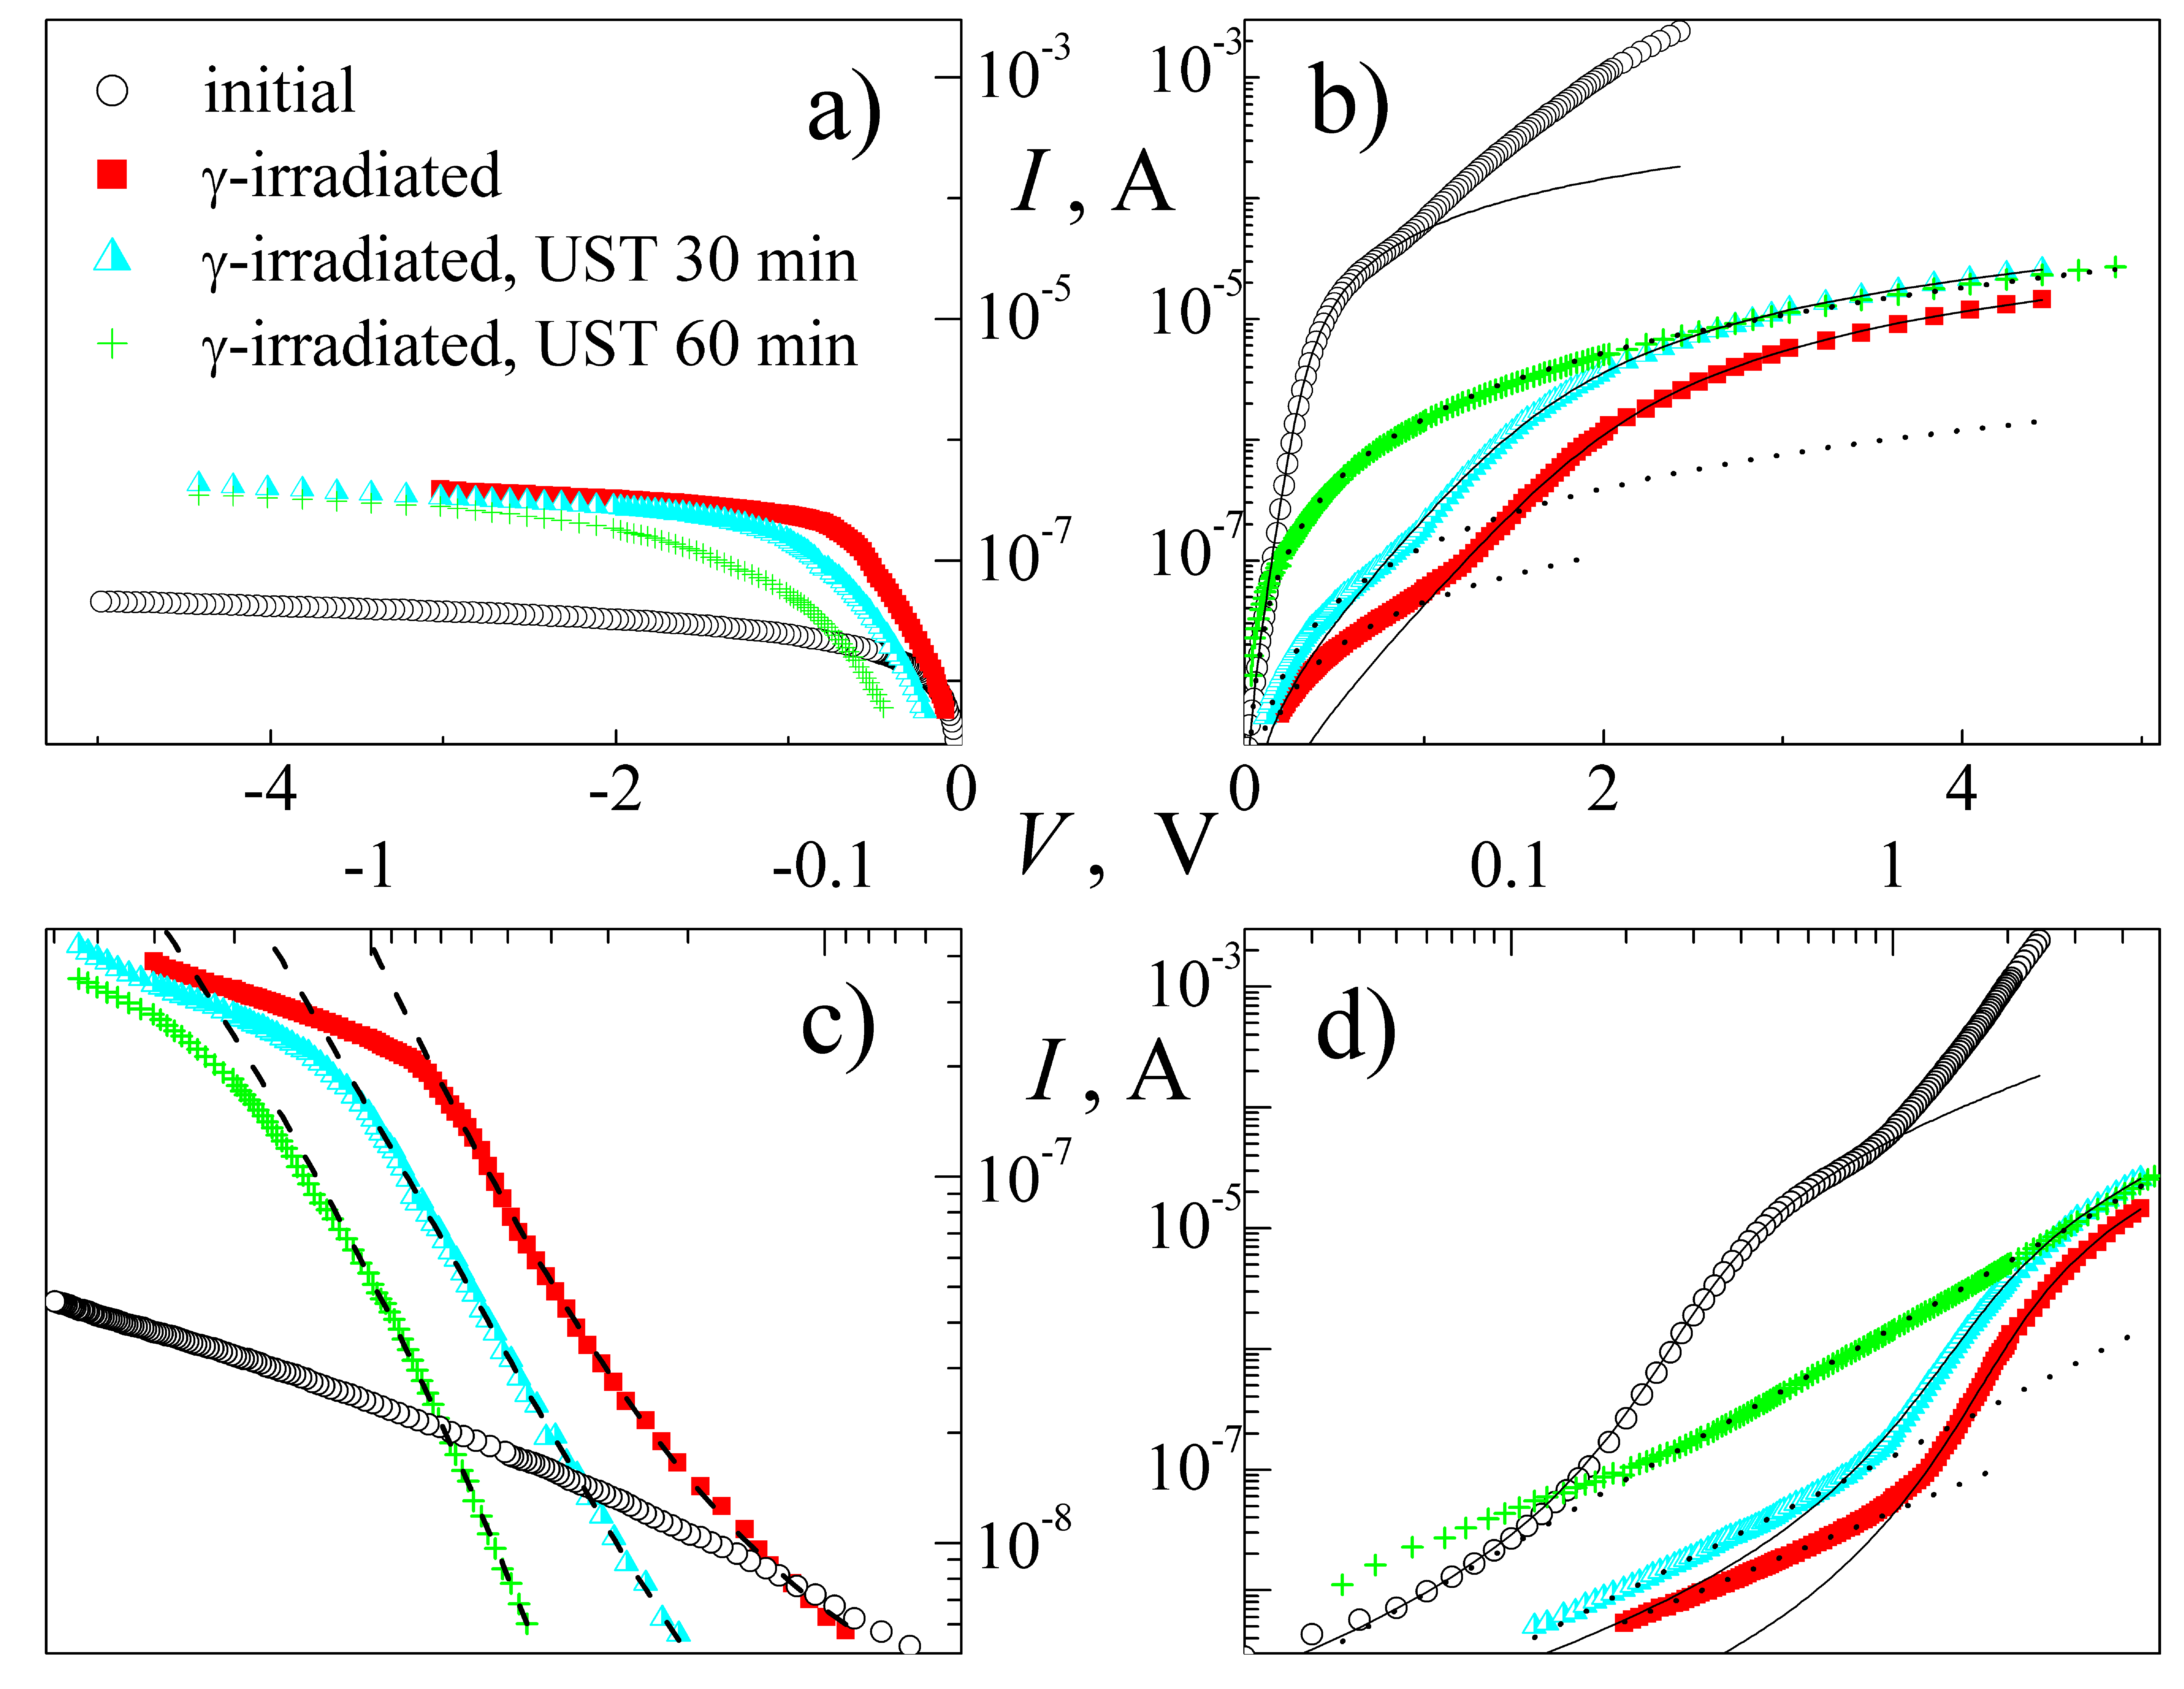
\includegraphics[width=0.95\textwidth]{figIV}}
\caption{\label{figIV}
The logarithmical (a, b) and double-logarithmical (c, d) plots of the reverse (a, c) and forward (b, d) $I$--$V$ characteristics for Au--SiO$_2$--Si structure before and after $\gamma$--irradiation and UST.
$T=300$~K.
The marks are the experimental results,
and the solid, dashed, and dotted lines are the TE, TAT, and SCLC fitted curves using Eqs.~(\ref{eqSDIV}), (\ref{eqIVTAT}), and (\ref{eqVIsclc}) respectively.
}%
\end{figure}




\begin{table}
\caption{\label{tabMIS}Extracted parameters for the Au--SiO$_2$--Si structure
}
\center
\begin{tabular}{lcccc}
\hline
\multicolumn{5}{l}{Structure status}\\\hline
$\gamma$--irradiation&$-$&$+$&$+$&$+$\\
UST&$-$&$-$&$+$&$+$\\
$t_\mathrm{UST}$ (min)&$0$&$0$&30&60\\ \hline
\multicolumn{5}{l}{Parameter}\\\hline
$I_s$ ($10^{-9}$A) & $3.3\pm0.3$& $1.1\pm0.2$& $4.9\pm0.5$&$-$ \\
$R_s$ ($10^{4}$��) & $1.1\pm0.2$& $13\pm1$& $9\pm1$&$-$ \\
$n$ & $1.7\pm0.1$& $10.3\pm0.2$& $9.9\pm0.2$& \\
$m_\mathrm{F}$ &$-$ &$1.30\pm0.05$& $1.6\pm0.05$& $1.8\pm0.05$ \\
$I_0$ ($10^{-8}$A) &$-$ &$5\pm1$& $13\pm2$& $150\pm10$ \\
$I_{0,\mathrm{TAT}}$ (a.u.) &$-$ &1& $0.14\pm0.03$& $0.04\pm0.01$ \\
$U_d$ (V) &$-$ &$0.7\pm0.1$& $0.44\pm0.05$& $0.12\pm0.05$ \\
$R_\mathrm{TAT}$ (a.u.) & &1& $0.54\pm0.05$& $0.33\pm0.04$ \\
$K_{\mathrm{RECT},\,\,0.5\mathrm{V}}$ &$800\pm100$ &$0.22\pm0.03$& $1.3\pm0.2$& $5.4\pm0.8$ \\
\end{tabular}
\end{table}

The experimental forward current value for the non--irradiated structure exceeds one, expected from Eq.~(\ref{eqSDIV}) at high bias --- see Fig.~\ref{figIV}.
The extra current is most likely to be caused by the tunneling through the SiO$_2$ layer.
The tunneling current can be given by \cite{Rhoderick1988,Novikov2009}:
\begin{equation}\label{eqFowlNord}
    \ln\left(\frac{I}{F_m^2}\right)\propto -\frac{4 \sqrt{2m^*}(qE_{\mathrm{eff}})^{3/2}}{3\hbar q F_m}\,,
\end{equation}
where
$F_m$ is the electric field,
$E_{\mathrm{eff}}$ is the effective tunneling energy.
%This assumption benefit is the linearity of the Fowler--Nordheim plots of the forward current at large bias --- see Fig.~\ref{FigFauler}.
The linearity of the Fowler--Nordheim plot (Fig.~\ref{FigFauler})  indicates  of reasonable assumption excess current mechanism.
It was taken into account when plotting that the electric field in a oxide layer is proportional to the applied voltage $F_m\propto V$.

\begin{figure}
\centerline{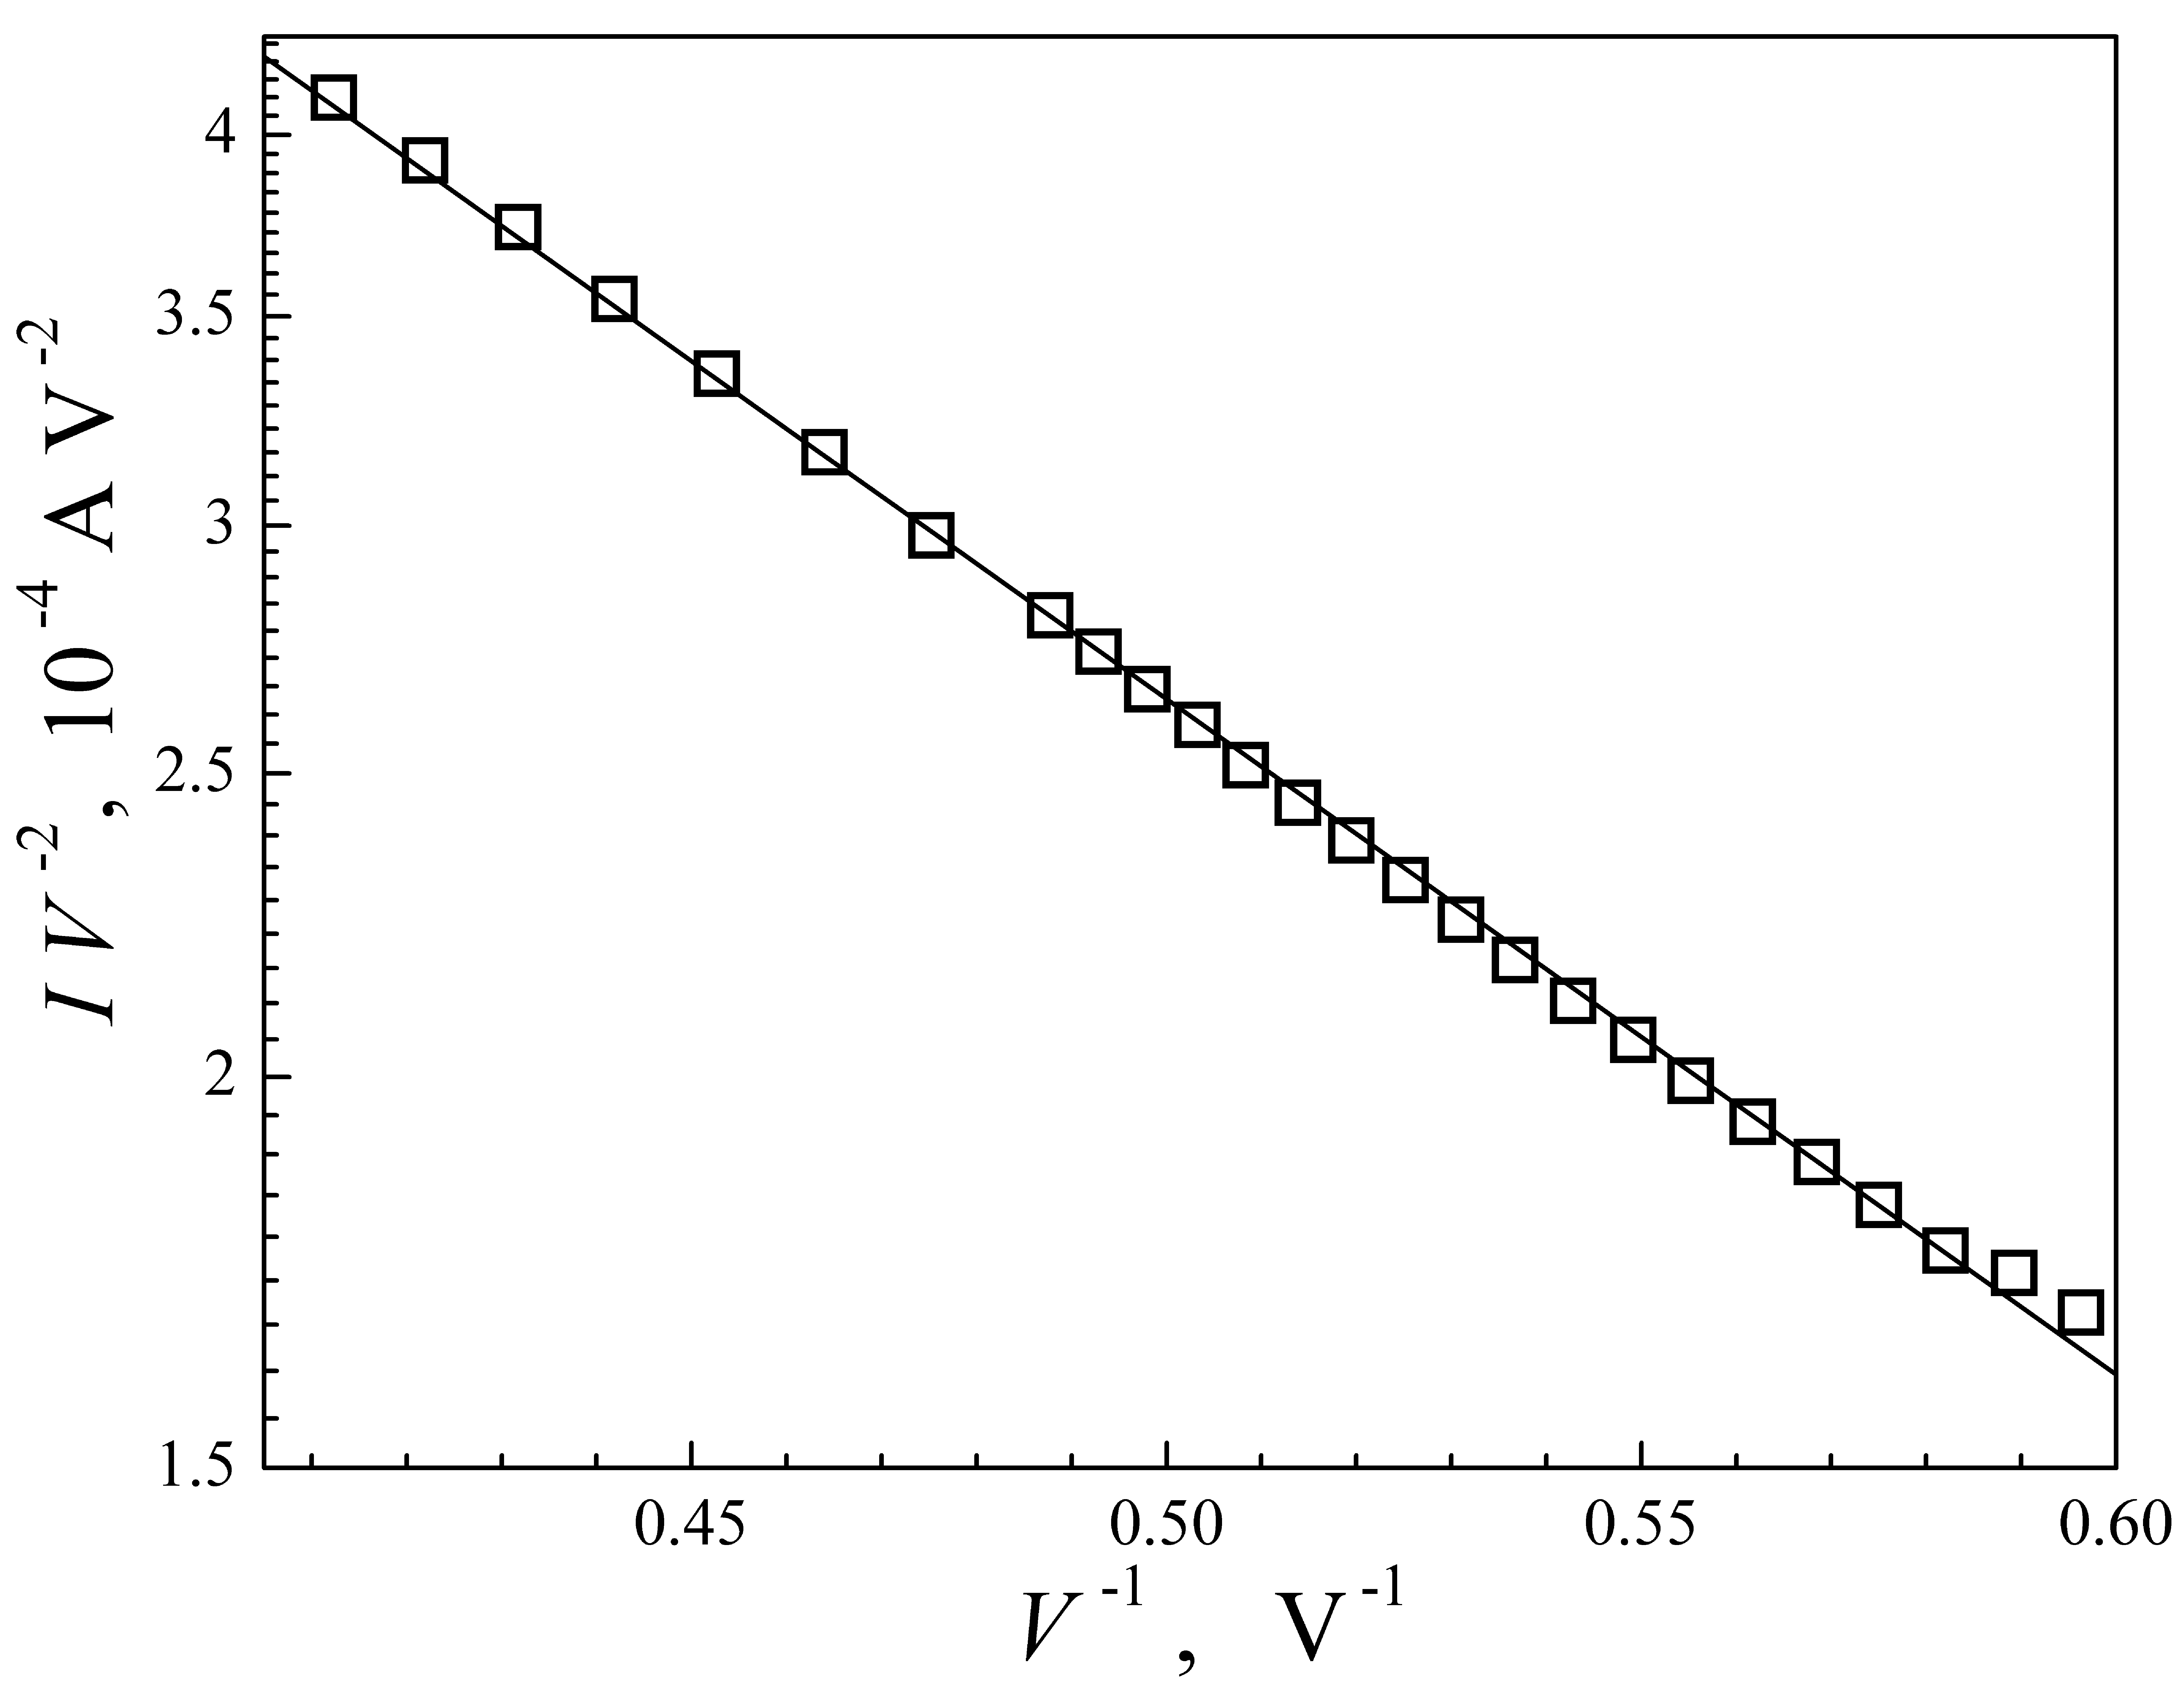
\includegraphics[width=0.6\textwidth]{FigFauler}}
\caption{\label{FigFauler}
The Fowler-Nordheim plot of the forward branch for non--irrradiated Au--SiO$_2$--Si structure at $V>1,6$~V.
The line is the least--squares linear fitting.
}%
\end{figure}

As shown in Fig.~\ref{figIV}, the $\gamma$--irradiation has a considerable effect on the current behavior.
% and the changes are especially pronounced in reverse branch.
The $I$--$V$ curve modification is evidence of transformation of current mechanism.
Thus the forward current decreased after irradiation and the $I$--$V$ dependence, which expected in TE model, is observed at $V>1$~V only.
Note that the effect of the radiation induced reduction of current in MOS structure was reported previously \cite{SiO2:Niu} as well.


The fitting of the $V>1$~V region by Eq.~(\ref{eqSDIV}) shown that the irradiation has caused significant increase in both series resistance value and ideality factor  --- see Table~\ref{tabMIS} data.
%And the former significantly exceeds the resistance change, which has been observed in the bulk samples.
In our opinion, $R_s$ increase deals with $\gamma$ influence on bulk Si.
Pintilie \emph{et al}. \cite{FZSi:Rad} investigated influence of $\gamma$-radiation ($9\cdot10^7$~rad) on silicon (Fz--Si, $4$~k$\Omega\cdot$cm).
It is shown that complexes VO$_i$, C$_i$C$_s$, $H$--center (V$_2$O$_i$), $\Gamma$--center, and interstitial defect $I^{0/-}$ are the main radiation defects.
%Pintilie \emph{et al}. \cite{FZSi:Rad} shown that complexes VO$_i$, C$_i$C$_s$, $H$--center (V$_2$O$_i$), $\Gamma$--center, and interstitial defect $I^{0/-}$ are the main defects, created by $^{60}$Co $\gamma$-radiation in Si.
%It should be noted that the growth method and resistivity of crystal, investigated in \cite{FZSi:Rad}, were analogous to our case; besides, the close doze ($9\cdot10^7$~rad) was used.
$I^{0/-}$ is a secondary defect and its appearance leads to conductivity compensation (inversion) \cite{FZSi:Rad}.
In our opinion, this defect is responsible for series resistance alteration.
In turn, significant increase in $R_s$ value (by 13 times) causes the reduction of voltage drop in the dielectric layer.
As a result, the electric field intensity was ceased to be sufficient for effective Fowler--Nordheim tunneling and such current component was not observed after irradiation.
The ideality factor increase deals with RD formation  as well and results in the observed decreasing of TE current.


Fig.~\ref{figIV}(d) shows that the forward $I$--$V$ characteristic of irradiated structures at low biases ($V<1$~V) is enough good described by a power law
\begin{equation}\label{eqVIsclc}
  I=I_0\,V^{\,m_\mathrm{F}},
\end{equation}
where
$m_\mathrm{F}=\frac{V}{I}\frac{\partial V}{\partial I}$ is the power--law parameter.
The relation (\ref{eqVIsclc}) is typical for the space charge limited current
(SCLC) \cite{SCLC:MA2016,Jafar,SCLC:Kaya} and $m_\mathrm{F}$ value deals with the energy distribution of traps, emitting carriers.
For instance, the value $m_\mathrm{F}\approx1.3$, which is observed for the investigated structure after $\gamma$--irradiation and before UST, is evident of the exponentially distributed traps.
It is known \cite{SCLC:MA2016,Jafar,SCLC:Kaya} that $I_0$ depends on the total trap concentration $N_t$
\begin{equation}\label{eqIoSCLC}
  I_0\sim 1/N_t^{m_\mathrm{F}-1},
\end{equation}
and the temperature dependency of  power--law parameter is given by
\begin{equation}\label{eqMT_IoSCLC}
  m_\mathrm{F}=1+T_c/T,
\end{equation}
where
$T_c$ is the parameter of trap energy distribution;
$P(E)=\frac{N_t}{kT_c}\exp(-\frac{E}{kT_c})$
is the trap concentration per unit energy range at an energy $E$ above the valence band.
The detect linearity of temperature dependence of $m_\mathrm{F}$ corroborates assumption about SCLC presence --- see inset in Fig.~\ref{figEa_MIS}.
In addition, it is known  \cite{Jafar} that the SCLC conduction should become important when the
density of injected carriers is much larger than the density of thermal--generated carrier.
Therefore SCLC appearance is enough expected in our case of high--resistance silicon substrate.


The SCLC current�--voltage relation is often written as \cite{Jafar}
\begin{equation}\label{eqVIsclcT}
  I(V,T)=C\exp\left(-\frac{E_x}{kT}\right)\,V^{\,m_\mathrm{F}(T)},
\end{equation}
where
$C$ is the constant,
$E_x$ is the activation energy linked to trap level.
Fig.~\ref{figEa_MIS} shows the temperature dependence of the forward current.
Eq.~(\ref{eqMT_IoSCLC}) was taken into account when Fig.~\ref{figEa_MIS} plotting.
It is seen that the experimental data are in good agreement with the fitting curve by Eq.~(\ref{eqVIsclcT}) for value $E_x=(0,32\pm0,01)$~eV.




\begin{figure}
\centerline{
\includegraphics[width=0.6\textwidth]{figEa_MIS}}
\caption{\label{figEa_MIS}
Temperature dependence of SCLC--current for $\gamma$--irrradiated Au--SiO$_2$--Si structure before UST at $V=0,4$~V.
Inset: Temperature dependence of power--law parameter.
Lines are the least--squares linear fitting.
}%
\end{figure}


Let's consider radiation defects, which is able to results in SCLC appearance.
First of all, some notes should be done.
Firstly, the low temperature and low partial oxygen pressure result in formation of thin SiO$_2$ layer in our case.
But same radiation defects are known \cite{SiO2:Cantin} to be  created in both thin and thick layers.
Secondly, the hydrogen content is the key factor of a  generation of electrically active RDs in Si---MOS structures \cite{SiO2:Cantin}.
But native SiO$_2$ layers are rich in an atomic hydrogen \cite{angermann2016,PersenkovBook}.


The $\gamma$--irradiation of Si--SiO$_2$ structures is known \cite{PersenkovBook} to lead to
a mechanical stress relaxation, a trap filling, and a charged defect generation.
It is believed \cite{SiO2:Devine,SiO2:Lenahan} that the negative charge is trapped at the interface while the positive charge accumulates in the oxide bulk.
In particular, the irradiation results in breaking of $\equiv\!\mathrm{Si}\!-\!\mathrm{H}$ bonds at Si--SiO$_2$ interface \cite{SiO2:Mahapatra,SiO2:Esseni,Fleetwood}.
The unsaturated bonds $\equiv\mathrm{Si}-$ act as electronic traps.
The configuration of such defects depends on orientation of silicon substrate.
It is considered \cite{SiO2:Rev} that $P_b$ centers appear at (111)--oriented substrate interface whereas $P_{b1}$ and $P_ {b0}$ centers are typical in the case of (100)--oriented substrate.
Both $P_ {b0}$ and $P_{b1}$ are chemically identical to the $P_b$,
however the difference in an electrical activity is observed \cite{SiO2:Rev}.
The  temperature of $P_b$ annealing is about 150$^\circ$C \cite{Fleetwood}.

The $\gamma$--ray irradiation with dose above $5\cdot10^5$~rad leads to non--monotonic energy distribution of interface levels in  $n$--Si---SiO$_2$ structure \cite{PersenkovBook}.
According to Parchinskii, \emph{et al}. \cite{ParchSiO2}, the highest density of surface states is observed at $E_c-(0,32\pm0,04)$~eV.
This value coincides with the determined  $E_x$ value.


In our opinion, the $P_b$ traps, being main electronic traps, are involved in SCLC process at low forward bias in irradiated structure.
Besides, the negative charge accumulation at interface results in  both rise of  barrier height and decrease of TE current.
%But as mentioned above, the main reason of TE current reduction is the $n$ rise induced  by RDs generation at silicon near surface region.

Figs.~\ref{figIV}(b) and (d) show that
UST causes an increase in space charge limited current.
We used Eq.~(\ref{eqVIsclc}) to fit experimental $I$--$V$ curves of ultrasonically treated structures.
The obtained fitting parameters are summarized in Table~\ref{tabMIS}.
According to Eq.~(\ref{eqIoSCLC}), the detected increase in $I_0$ value is evident of AI decrease in $P_b$ concentration.
It should be pointed out that acousto--annealing takes place at low (about~80$^\circ$C) temperature.

On the one hand,
the acousto-�defect interaction in Si is observed \cite{Roman:2010JAP,Korotchenkov1995,Olikh2009Sem,UST:Medvid,OlikhJAP,Savkina2015}
to cause atomic diffusion, transformation of native and impurity defects,
modification of interior surface states, and appearance of new defects.
On the other hand,
the $P_b$ center annealing is known \cite{SiO2:Takakura,SiO2:Wurzer} to deal with the passivation of dangling bonds at the oxide--silicon interface by hydrogen atoms.
Thus obtained results indicate about AI diffusion of hydrogen.
Similar phenomenon is previously reported \cite{Ostap:SiO2,Ostap:PhotoLum,ostapenko1997},
but this is a way of acousto--annealing of radiation defects in our case.


Table~\ref{tabMIS} shows that UST leads to increase in $m_\mathrm{F}$ value.
According to Eq.~(\ref{eqMT_IoSCLC}), the $m_\mathrm{F}$ increment deals with  increase in $T_c$ value as well as narrowing of distribution of trap level.
So, it is known \cite{Jafar} that $m_\mathrm{F}=2$ is observed in the case of single--energy trap.
The detected narrowing is evidence of acousto--annealing selectivity,
that is, UST leads to atomic hydrogen capture by certain dangling bonds only.
In our opinion, the key parameter of the AI bond passivation is a mechanical stress, which are generally non--uniform at the interface.
The impurity diffusivity is known \cite{AZIZ2001} to depend on mechanical stress.
On the one hand, change of mechanical stress can be an reason of hydrogen displacement under acoustic loading condition.
On the other hand, the efficiency of AI passivation is determined by a value of mechanical deformation around defect.

The acousto--annealing of $P_b$ centers lead to the decrease in interface negative charge
and results in  both partial recovery of barrier height and increase in TE current value --- see Table~~\ref{tabMIS}.
The detected AI decrease in $R_s$ value is evidence of RD ($I^{0/-}$ center) annealing in silicon bulk.



The $\gamma$--released hydrogen is potentially hazardous because of this  mobile  species  is able \cite{SiO2:Devine,SiO2:DiMaria,SiO2:Mahapatra,SiO2:Esseni}
i)~to interact with bonded hydrogen at Si/SiO$_2$  interface  and to give rise to additional $P_b$ centers;
ii)~to move to semiconductor bulk and to produce generation--recombination  sites  and boron  deactivation in  the Si  substrate;
iii)~to migrate within oxide and to create $E'$ centers.
It is believed \cite{SiO2:Takakura,SiO2:Devine} that $E'$ center is due to broken $\equiv\!\mathrm{Si}\!-\!\mathrm{O}$ bonds,
results from an oxygen vacancy in SiO$_2$, and traps positive charge.
It is concluded \cite{Fleetwood,SiO2:Devine} that $E'$ centers dominate hole trapping in a oxide films on silicon.
The  $E'$ total concentration is about $10^{18}$~cm$^{-3}$ in the case of $10^{7}$~rad $\gamma$--irradiation, but centers are non--uniformly distributed over oxide layer depth and
largest concentration are expected near Si/SiO$_2$  interface  \cite{PersenkovBook}.
The broken $\equiv\!\mathrm{Si}\!-\!\mathrm{O}$ bonds does not recover at room temperature and the  temperature of $E'$ annealing is equal 200$^\circ$C \cite{SiO2:Mahapatra,SiO2:Takakura,Fleetwood}.

A generation of $E'$ centers are accompanied by a large (several orders of magnitude) increase in leakage currents \cite{SiO2:Mahapatra,SiO2:DiMaria,Fleetwood}.
The leakage currents are likely caused by inelastic tunneling of conduction band electrons to defect centers in the oxide near the  Si/SiO$_2$ boundary \cite{Fleetwood,SiO2:Esseni,SiO2:DiMaria}.
In our opinion, such trap--assisted tunneling (TAT) current is responsible for a reverse current in irradiated structures --- Figs.~\ref{figIV}(a) and \ref{figIV}(c).

In fact, according to \cite{TAT:Gilmore,TAT:GopalSST,TAT:Gopal}, the bias dependence of TAT current is described as
\begin{equation}\label{eqIVTAT}
  I_R=I_{0,\mathrm{TAT}}\,(U_d-V)\exp\left(-\frac{R_\mathrm{TAT}}{F_m}\right),
\end{equation}
where
$I_{0,\mathrm{TAT}}$ and $R_\mathrm{TAT}$ do not depend on voltage,
$I_{0,\mathrm{TAT}}$ is proportional to trap concentration;
$U_d$ is the barrier height.
The reverse $I$--$V$ branches of irradiated structure before and after UST were fitted by using Eq.~(\ref{eqIVTAT}) --- see Fig.~\ref{figIV}.
The experimental data are in good agreement with the fitting curves.
The fitting results confirm assumption about the reverse current mechanism.
The current deviation at high bias is probably caused by series resistance.


Determined parameters are listed in Table~\ref{tabMIS}.
It is seen that UST leads to decrease in $I_{0,\mathrm{TAT}}$ and barrier height values.
The former is evidence of low temperature acousto--annealing of radiation traps ($E'$ center).
The acoustically stimulated diffusion of interstitial oxygen and hydrogen atoms is most likely reason of $E'$ annealing.
The barrier lowering are in agreement with $P_b$ annealing, mentioned above.


The investigation shows that $\gamma$--irradiation results in considerable degradation of  rectification factor $K_\mathrm{RECT}$.
But UST leads to a forward current increase as well as reverse current decrease in irradiated  Au�-SiO$_2$�-Si structure.
Therefore  $K_\mathrm{RECT}$ is recovered by an acoustic wave action.
The $K_\mathrm{RECT}$ data at 0.5~V are listed in Table~\ref{tabMIS}.
Thereby, the possibility of partial recovery of properties of $\gamma$--degraded Si--MOS structure by ultrasound treatment at close to room--temperature is shown.


\section{Conclusion}
The experimental investigation of influence of $\gamma$--irradiation and ultrasound treatment on current mechanism in Au�-SiO$_2$�-Si structure has been carried out.
The thermionic emission and tunneling through the SiO$_2$ layer were a main reason of current in initial structure.
It has been shown that $\gamma$--irradiation results in origin of space charge limited current at forward bias and trap--assisted tunneling current at reverse bias as well as in attenuation of TE current.
%The irradiation influence deals with negative charge trapping by $P_b$ centers  at interface and creation of $E'$ centers in oxide bulk.
The investigation has revealed that ultrasound treatment at close to room--temperature leads to increase in rectification factor value.
The acoustically induced variation of current value is indicative of low--temperature (80$^\circ$C) annealing of $P_b$ and $E'$ centers.
The  most likely reason of detected effect is enhance of diffusivity of interstitial species (hydrogen and oxygen) under ultrasound loading condition.
In addition, by relying  on increase in the value of power--law parameter of a space charge limited current,
it has been concluded that ultrasound treatment leads to narrowing of energy distribution of $\gamma$--induced traps at Si/SiO$_2$  interface.
Thus, ultrasound can be an effective tool for controlling metal�-semiconductor structure characteristics.


\bibliography{olikh}

\end{document}

